%%%%%%%%%%%%%%%%%%%%%%%%%%%%%%%%%%%%%%%%%
% baposter Landscape Poster
% LaTeX Template
% Version 1.0 (11/06/13)
%
% baposter Class Created by:
% Brian Amberg (baposter@brian-amberg.de)
%
% This template has been downloaded from:
% http://www.LaTeXTemplates.com
%
% License:
% CC BY-NC-SA 3.0 (http://creativecommons.org/licenses/by-nc-sa/3.0/)
%
%%%%%%%%%%%%%%%%%%%%%%%%%%%%%%%%%%%%%%%%%

%----------------------------------------------------------------------------------------
%	PACKAGES AND OTHER DOCUMENT CONFIGURATIONS
%----------------------------------------------------------------------------------------

\documentclass[landscape,a0paper,fontscale=0.31]{baposter} % Adjust the font scale/size here

\usepackage{graphicx} % Required for including images
\graphicspath{{figures/}} % Directory in which figures are stored

\usepackage{amsmath} % For typesetting math
\usepackage{amssymb} % Adds new symbols to be used in math mode

\usepackage{breqn}  % Used for breaking equations on multiple lines


\usepackage{booktabs} % Top and bottom rules for tables
\usepackage{enumitem} % Used to reduce itemize/enumerate spacing
\usepackage{palatino} % Use the Palatino font
\usepackage[font=small,labelfont=bf]{caption} % Required for specifying captions to tables and figures

\usepackage{multicol} % Required for multiple columns
\setlength{\columnsep}{1.5em} % Slightly increase the space between columns
\setlength{\columnseprule}{0mm} % No horizontal rule between columns

\usepackage{tikz} % Required for flow chart
\usetikzlibrary{shapes,arrows} % Tikz libraries required for the flow chart in the template

\newcommand{\compresslist}{ % Define a command to reduce spacing within itemize/enumerate environments, this is used right after \begin{itemize} or \begin{enumerate}
\setlength{\itemsep}{1pt}
\setlength{\parskip}{0pt}
\setlength{\parsep}{0pt}
}

\definecolor{lightblue}{rgb}{0.145,0.6666,1} % Defines the color used for content box headers

\begin{document}

\begin{poster}
{
headerborder=closed, % Adds a border around the header of content boxes
colspacing=1em, % Column spacing
bgColorOne=white, % Background color for the gradient on the left side of the poster
bgColorTwo=white, % Background color for the gradient on the right side of the poster
borderColor=lightblue, % Border color
headerColorOne=black, % Background color for the header in the content boxes (left side)
headerColorTwo=lightblue, % Background color for the header in the content boxes (right side)
headerFontColor=white, % Text color for the header text in the content boxes
boxColorOne=white, % Background color of the content boxes
textborder=roundedleft, % Format of the border around content boxes, can be: none, bars, coils, triangles, rectangle, rounded, roundedsmall, roundedright or faded
eyecatcher=true, % Set to false for ignoring the left logo in the title and move the title left
headerheight=0.1\textheight, % Height of the header
headershape=roundedright, % Specify the rounded corner in the content box headers, can be: rectangle, small-rounded, roundedright, roundedleft or rounded
headerfont=\Large\bf\textsc, % Large, bold and sans serif font in the headers of content boxes
%textfont={\setlength{\parindent}{1.5em}}, % Uncomment for paragraph indentation
linewidth=2pt % Width of the border lines around content boxes
}
%----------------------------------------------------------------------------------------
%	TITLE SECTION 
%----------------------------------------------------------------------------------------
%
{
\includegraphics[height=4em]{JACOBS_LOGO.jpg}} % First university/lab logo on the left
{\bf\textsc{Bound states in the continuum}} % Poster title
{\textsc{ Daniel Prelipcean \\  Jacobs University Bremen \\   Department of Physics and Earth Sciences}} % Author names and institution
{
\includegraphics[height=4em]{JACOBS_LOGO.jpg}} % Second university/lab logo on the right



%----------------------------------------------------------------------------------------
%	INTRODUCTION
%----------------------------------------------------------------------------------------

\headerbox{Introduction}{name=introduction,column=0,row=0}{


In 1929, von Neumann and Wigner claimed \cite{ref2} that the single-particle Schr{\"o}dinger equation could possess isolated eigenvalues embedded in the continuum of positive energy states. They offered a constructive method based upon amplitude modulation of a free-particle wave function and leading to a localized (i.e., integrable) eigenfunction and a local potential which produces it. The potential was bounded and could be made to vanish at infinity. Diffractive interference was proposed as the reason such localized positive-energy states could exist.


}

%----------------------------------------------------------------------------------------
%	OBJECTIVES
%----------------------------------------------------------------------------------------

\headerbox{Objectives}{name=objectives,column=0,row=1,below=introduction}{

The aim of Stillinger and Herricks`s paper \cite{ref1} was to construct quantum-mechanical examples with local potentials that allow bound eigenstates embedded in the dense continuum of scattering states.\\

In the light of the Further Examples section, attention is focused on quantitative interpretation of real tunneling phenomena, and on the existence of continuum bound states in atoms and molecules.



\vspace{0.3em} % When there are two boxes, some whitespace may need to be added if the one on the right has more content
}

%----------------------------------------------------------------------------------------
%	Results
%----------------------------------------------------------------------------------------

\headerbox{Graphical Results}{name=results,column=2,span=2,row=0}{
\begin{multicols}{2}
\vspace{1.5cm}
\begin{center}
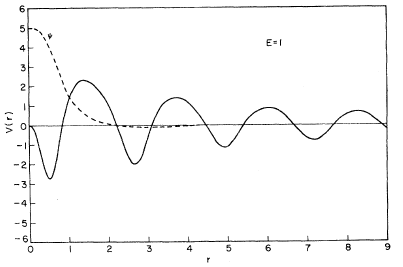
\includegraphics[width=0.98\linewidth]{figures/Potential1.PNG}
\captionof{figure}{Potential-energy function for particle energy l.  \cite{ref1} Classically, the particle would have been trapped inside the potential barrier since its energy is lower than the barrier. }
\end{center}

\begin{center}
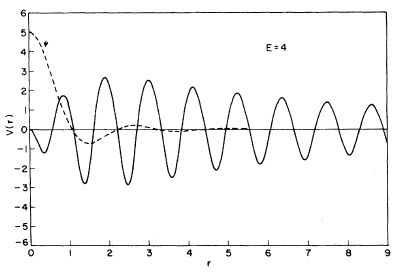
\includegraphics[width=1.0\linewidth]{figures/Potential.PNG}
\captionof{figure}{Potential-energy function with energy 4. \cite{ref1} This energy exceeds the maximum value
for the potential, so the particle could not be trapped even by classical mechanics.}
\end{center}	

\end{multicols}
}

%----------------------------------------------------------------------------------------
%	REFERENCES
%----------------------------------------------------------------------------------------

\headerbox{References}{name=references,column=0,span=2,above=bottom}{

\renewcommand{\section}[2]{\vskip 0.05em} % Get rid of the default "References" section title
\nocite{*} % Insert publications even if they are not cited in the poster
\small{ % Reduce the font size in this block
\bibliographystyle{unsrt}
\bibliography{sample} % Use sample.bib as the bibliography file
}}

%----------------------------------------------------------------------------------------
%	FUTURE RESEARCH
%----------------------------------------------------------------------------------------

\headerbox{Ongoing Research}{name=ongoingresearch,column=2,span=2, above=bottom}{ 
The very existence of Bound States in Continuum defies conventional wisdom. Although first proposed in quantum mechanics, they are a general wave phenomenon and have since been identified in electromagnetic waves, acoustic waves in air, water waves and elastic waves in solids. These states have been studied in a wide range of material systems, such as piezoelectric materials, dielectric photonic crystals, optical waveguides and fibres, quantum dots, graphene and topological insulators.
}

%----------------------------------------------------------------------------------------
%	Further examples
%----------------------------------------------------------------------------------------

\headerbox{Further Examples}{name=furtherexamples,column=2,span=1,row=0,below=results, above = ongoingresearch}{
These examples involve just single particles, furthermore, they can be reduced to one-dimensional form by virtue of separability:
\begin{enumerate}
\item[A] Higher angular momentum: for a free-particle state with total-angular-momentum quantum number $l$;  $\psi^{(l)} = f_l(r) R_l (kr) Y_{lm}(\theta, \phi) $

\item[B] Variable dimensionality: ground state of the helium isoelectronic sequence for variable dimensionality.
\item[C] Coulomb interactions (only for repulsive potentials)
\item[D] Constant electric field (potential linear in displacement along the field)
\end{enumerate}

The non-separable case is given by the Doubly Excited atom: a model "two-electron" atom which, with suitable
interaction between the electrons, will have a
doubly excited state with infinite lifetime (within
the Schr{\"o}dinger description).

\vspace{2em}

}


%----------------------------------------------------------------------------------------
%	Discussion
%----------------------------------------------------------------------------------------

\headerbox{Discussion}{name=conclusion,column=3,span=1,row=0,below=results, above = ongoingresearch}{
The eigenvalue for the preceding positive-energy bound state can be moved up or down within the continuum merely by varying the wave vector $k$. Equation \ref{potential} specifies the way in which $V(r)$ must deform to continue supporting its bound state nature.\\

The examples of continuum bound states constructed by Stillinger and Herrick \cite{ref1} sent a warning against quantitative over-interpretation of the tunneling phenomena: 
\begin{enumerate}
\item Cold emission of electrons from metals, under the influence of strong electric fields,
\item Alpha decay rates of radioactive nuclei,
\item Tunneling through films between adjacent solid phases.
\end{enumerate}

If a given physical system were to possess a potential close to the subspace of potentials with continuum bound states, then its tunneling rate would be anomalously small. 
}

%----------------------------------------------------------------------------------------
%	Definitions
%----------------------------------------------------------------------------------------

\headerbox{Definitions}{name=definitions,column=0,below=objectives,above=references}{ % This block's bottom aligns with the bottom of the conclusion block

Bound state = a bound state is a special quantum state of a particle subject to a potential such that the particle has a tendency to remain localized in one or more regions of space. \\

Continuum =  matter continuously distributed and fills the entire region of space it occupies. Here, continuum is considered to be wave functions with positive energies, compared to bound states with negative energies.\\

Node = a point along a standing wave where the wave has minimum (usually vanishing) amplitude.\\

Separability = the wave function can be written as a direct product of individual wave functions. Usually the case for non-interacting particles.

}

%----------------------------------------------------------------------------------------
%	Procedure
%----------------------------------------------------------------------------------------

\headerbox{Von Neumann-Wigner Method}{name=results2,column=1,row=0,above=references}{ % 

In natural units, the single-particle Schr{\"o}dinger wave equation is to be solved in infinite three-space:
\begin{equation}
\left( - \frac{1}{2} \nabla^2 + V \right) \psi = E \psi
\label{schreq}
\end{equation}

Momentarily, we consider only bounded potentials V, and which are local operators in position representation. Eqn. \ref{schreq} can be reversed to obtain the potential,
\begin{equation}
V = E + \frac{1}{2} \left( \frac{\nabla^2 \psi}{\psi} \right)
\end{equation}
which implies that the nodes of the wave function $\psi$ must be matched by vanishing of its Laplacian.
For $V=0$, the free particle S-wave,
\begin{equation}
\psi_0 (r) = \sin{(kr)}/kr
\end{equation}
satisfies the above with energy eigenvalue $E = k^2/2$. To obtain potentials yielding bounded states, consider an amplitude modulation $f(r)$ and $\psi(r) = \psi_0 (r) f(r)$.
\begin{equation}
V(r) = E - \frac{1}{2}k r^2 + k \cot(kr) \frac{f'(r)}{f(r)} + \frac{1}{2}\frac{f''(r)}{f(r)}
\end{equation}
Further constrains are needed for the envelop function $f(r)$ to keep the potential bounded. The specific choice suggested by von Neumann and Wigner \cite{ref2} is:
\begin{equation}
f(r) = \{ A^2 + [ 2kr - \sin{2kr} ]^2 \}^{-1}
\end{equation}
where $A$ is an arbitrary nonzero constant. Thereby:
\begin{dmath}
V(r) = - \frac{64 k^2 A^2 \sin^4 (kr)}{[A^2 + (2kr - \sin (2kr)^2]^2} + \frac{48 k^2 \sin ^4 kr - 8k^2 (2kr - \sin 2kr)}{A^2 + (2kr - \sin 2kr)^2 }
\label{potential}
\end{dmath}
Near the origin, the function reduces to:
\begin{equation}
V(r) = (80/3A^2 -64)k^2 (kr)^4 + O((kr)^6)
\end{equation}
while its large $r$ form is expressed as:
\begin{equation}
V(r) \sim -8k^2 (\sin 2kr)/2kr
\end{equation}

}

%----------------------------------------------------------------------------------------

\end{poster}

\end{document}